% Created 2016-04-28 tor 16:53
% Intended LaTeX compiler: pdflatex
\documentclass{scrartcl}
\usepackage[utf8]{inputenc}
\usepackage[T1]{fontenc}
\usepackage{graphicx}
\usepackage{grffile}
\usepackage{longtable}
\usepackage{wrapfig}
\usepackage{rotating}
\usepackage[normalem]{ulem}
\usepackage{amsmath}
\usepackage{textcomp}
\usepackage{amssymb}
\usepackage{capt-of}
\usepackage{hyperref}
\usepackage{khpreamble}
\newcommand{\tustin}{\frac{2}{h}\frac{z-1}{z+1}}
\author{Kjartan Halvorsen}
\date{2015-11-24}
\title{Computerized control - Final Exam - modified from Fall 2015}
\hypersetup{
 pdfauthor={Kjartan Halvorsen},
 pdftitle={Computerized control - Final Exam - modified from Fall 2015},
 pdfkeywords={},
 pdfsubject={},
 pdfcreator={Emacs 24.5.1 (Org mode 8.3.4)}, 
 pdflang={English}}
\begin{document}

\maketitle
The dynamic model of a ship with input \(u\) being the rudder angle and the output \(y\) being the heading (see figure \ref{fig:tanker}) can be described as a continuous-time second order system with a pole in the origin
\[ G(s) = \frac{K}{s(s + a)}. \]
For fully loaded, large tankers this dynamics is often unstable, meaning that \(a<0\) \footnote{Fossen, Thor I. Handbook of marine craft hydrodynamics and motion control. John Wiley \& Sons, 2011.} .  
\begin{figure}[h]
\begin{center}
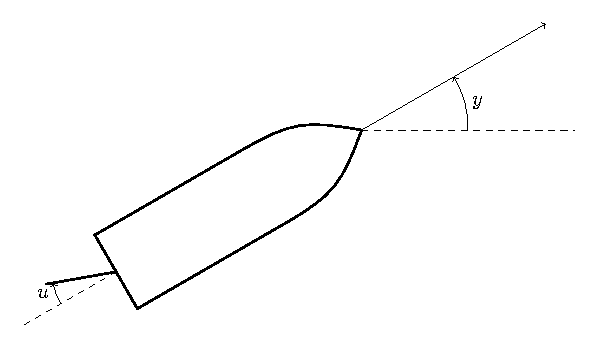
\includegraphics[]{tanker}
\caption{Heading of a ship controlled by rudder input.}
\label{fig:tanker}
\end{center}
\end{figure}

Consider for this exam the normalized continuous-time model of the tanker
\[ G(s) = \frac{1}{s(s - 1)}. \]
with the discrete-time model obtained by zero-order hold
\begin{equation*}
 H(z) = \frac{(-1+\mexp{h} -h)z + 1 - (1-h)\mexp{h}}{(z-1)(z-\mexp{h})}.
\end{equation*}
Specifically, use sampling time \(h=0.2\), which gives the (approximate) model
\begin{equation}
 H(z) = \frac{0.02z + 0.02}{(z-1)(z-1.2)} = \frac{0.02z + 0.02}{z^2-2.2z+1.2}.
\label{eq:model}
\end{equation}

\textbf{All answers should be well motivated!}

\section*{Problem 1}
\label{sec:orgheadline1}
\begin{enumerate}
\item In figure \ref{fig:complex-plane} draw the poles (crosses) and zero (circle) for the  discrete-time pulse-transfer function in \eqref{eq:model}.
\begin{figure}[h]
\begin{center}
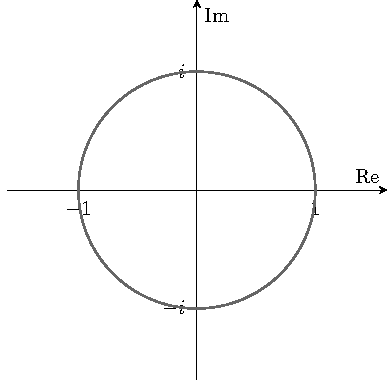
\includegraphics[]{complex-plane}
\caption{Problem 1: Plot the poles and zeros of the discrete-time system.}
\label{fig:complex-plane}
\end{center}
\end{figure}
\item Assume that the tanker with model \eqref{eq:model} is stabilized using error-feedback and a PD-controller. The  Bode-diagram of the resulting \textbf{closed-loop} system is  given in figure \ref{fig:bode}. What is the bandwidth of the closed-loop system? At what frequency is the resonance peak? 
\begin{figure}[h]
\begin{center}
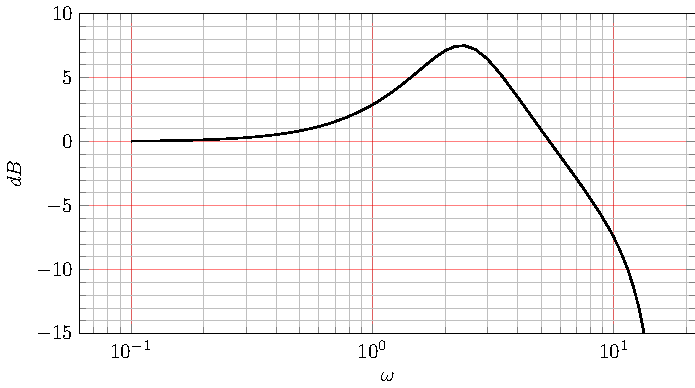
\includegraphics[]{bode-closed}
\caption{Problem 1: Bode diagram of closed-loop system with PD-control}
\label{fig:bode}
\end{center}
\end{figure}
\end{enumerate}

\section*{Problem 2}
\label{sec:orgheadline2}
Figure \ref{fig:rst} shows a system controlled with an RST controller. Note that the system includes an anti-aliasing filter modelled as a pure time-delay of two sampling periods. What is the closed-loop pulse-transfer function from the disturbance \(d\) to the output \(y\)? You do not need to multiply the polynomials. It is sufficient to state your answer in terms of \(A(z)\), \(B(z)\), \(R(z)\), \(S(z)\) and \(z^2\).
\begin{figure}[h]
\begin{center}
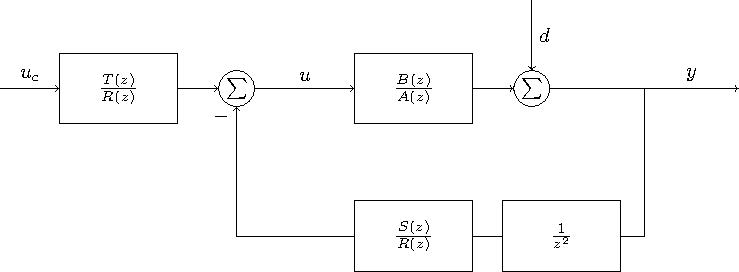
\includegraphics[]{rst-anti-aliasing}
\caption{Problem 2: Two-degree-of-freedom controller with anti-aliasing filter.}
\label{fig:rst}
\end{center}
\end{figure}


\section*{Problem 3}
\label{sec:orgheadline3}
When designing an RST-controller for the system in Problem 2, \(R(z)\) and \(S(z)\) are determined from a diophantine equation, based on the required placement of the closed-loop poles. Assume the following desired closed-loop denominator:
\begin{equation}
A_{cl} = \underbrace{(z-p_1)(z-p_2)z^2}_{A_c}\underbrace{(z-p_3)^3}_{A_o}
\end{equation}
\begin{enumerate}
\item Write the diophantine equation in terms of \(A_c(z)\), \(A_o(z)\), \(A(z)\), \(B(z)\), \(R(z)\), \(S(z)\) and \(z^2\).
\item Let the controller polynomials \(R(z)\) and \(S(z)\) have the same order. Determine this order, so that all the controller parameters can be determined from the diophantine equation. Note that you only need to determine the \textbf{order} of the controller. You do not need to write the equation for the controller parameters.
\end{enumerate}

\section*{Problem 4}
\label{sec:orgheadline4}
The controllable canonical state-space representation of \eqref{eq:model} is given by
\begin{equation}
\begin{split}
x(k+1) &= \bbm 2.2 & -1.2\\1 & 0\ebm \x(k) + \bbm 1\\0\ebm u(k)\\
y(k) &= \bbm 0.02 & 0.02 \ebm x(k),
\end{split}
\end{equation}
with 
\[ x(k) = \bbm x_1(k)\\x_2(k)\ebm. \]
Introduce the state-feedback law \(u(k) = -l_1x_1(k) -l_2x_2(k)\) and determine \(l_1\) and \(l_2\) so that the closed-loop system has the characteristic polynomial
\[ (z-0.9+0.1i)(z-0.9-0.1i) = z^2 -1.8z + 0.82. \]

\section*{Solution}
\label{sec:orgheadline9}
\subsection*{Problem 1}
\label{sec:orgheadline5}
\begin{enumerate}
\item Poles and zeros
\begin{center}
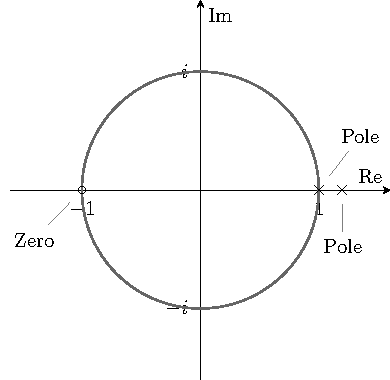
\includegraphics[]{complex-plane-sol-final}
\end{center}
\item Bandwidth and resonance
\begin{center}
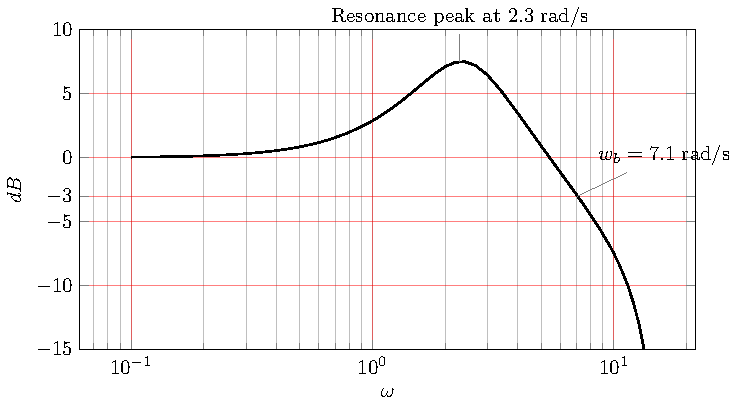
\includegraphics[]{bode-closed-sol}
\end{center}
\end{enumerate}

\subsection*{Problem 2}
\label{sec:orgheadline6}
To compute the pulse-transfer function from \(d\) to \(y\), assume \(u_c=0\). We get
\begin{equation*}
\begin{split}
Y &= D + \frac{B}{A} U = D - \frac{B}{A}\frac{S}{R}\frac{1}{z^2} Y\\
Y + \frac{BS}{ARz^2} Y &= D\\
Y &= \frac{1}{1 + \frac{BS}{ARz^2}} D\\
 &= \frac{A(z)R(z)z^2}{A(z)R(z)z^2 + B(z)S(z)} D
\end{split}
\end{equation*}

\subsection*{Problem 3}
\label{sec:orgheadline7}
\begin{enumerate}
\item The diophantine equation becomes
\[ A(z)R(z)z^2 + B(z)S(z) = A_c(z)A_o(z) \]
\item The right hand side of the diophantine equation has order 7, hence the left hand side must have the same order. Since \(A(z)z^2\) has order 4, then \(R(z)\) must have order 3. We choose \(R(z)\) and \(S(z)\) to have the same order (which is a smart choice because then the pulse-transfer function of the controller does not introduce a time-delay), we get
\[ \frac{S(z)}{R(z)} = \frac{s_0z^3 + s_1z^2 + s_2z + s_3}{z^3+r_1z^2 + r_2z + r_3} \]
which has 7 parameters. The diophantine equation gives 7 equations to determine uniquely the 7 control parameters. Note that the terms \(A(z)R(z)z^2\) and \(B(z)S(z)\) do \textbf{not} have to have the same order.
\end{enumerate}

\subsection*{Problem 4}
\label{sec:orgheadline8}
With the control law we get the closed-loop system 
\begin{equation*}
\begin{split}
 x(k+1) &= \bbm 2.2 & -1.2\\1 & 0\ebm x(k) - \bbm l_1 & l_2\\ 0 & 0 \ebm x(k)\\
        &= \bbm 2.2-l_1 & -1.2-l_2\\1 & 0\ebm x(k)
\end{split}
\end{equation*}
which is also on controllable canonical form. Thus we can immediately write the characteristic polynomial of the closed-loop system as 
\[ z^2 + (-2.2+l_1)z + (1.2 + l_2). \]
It is also straight-forward to write the characteristic polynomial using the formula
\begin{equation*}
\begin{split}
\det \left( zI - \bbm 2.2-l_1 & -1.2-l_2\\1 & 0\ebm \right) 
        &= \det \bbm z -2.2+l_1 & 1.2+l_2\\-1 & z\ebm\\
	&= (z-2.2+l_1)z + (1.2+l_2) = z^2 + (-2.2+l_1)z + (1.2+l_2).
\end{split}
\end{equation*}

Comparing coefficients with the desired characteristic polynomial 
\[ z^2 -1.8 + 0.82 \] gives the solution
\begin{align*}
l_1 &= -1.8 + 2.2 = 0.4\\
l_2 &= 0.82 - 1.2 = - 0.38
\end{align*}

With \[ m_0 = \frac{A_c(1)}{B(1)} = \frac{1-1.8+0.82}{0.02+ 0.02} = 0.5 \]
and 
\[ u = -Lx + m_0u_c, \]
the Bode-diagram of the closed-loop system becomes
\begin{center}
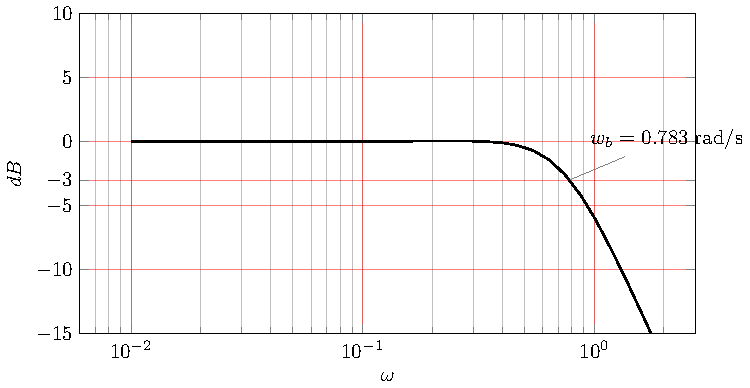
\includegraphics{bode-statefb-closed-sol}
\end{center}
\end{document}
